%%%TODO: explorar mais artigos recolhidos e ver zotero o que ja tenho, e criar mais ligacoes entre as frases e conceitos

%fayyad explorar mais e melhor intro
\ac{kdd} is about turning data into knowledge. However, turning data into knowledge or insights is not new in healthcare. The first attempts to use data to improve healthcare date back to the 17th century, when John Graunt used data from the London Bills of Mortality to study the causes of death in the city \cite{741e4dcd-5d3c-325c-9241-5eb5ddd0cb60}. This was the first time that data was used to understand the health of a population. Since then, the field of \ac{kdd} has evolved significantly, and it is now a crucial part of healthcare, helping to improve patient outcomes, enhance clinical decision-making, and optimize healthcare delivery.
Additionally, the fact that data is being collected at an unprecedented rate, and the need to extract knowledge from it, has led to the development of several methodologies and frameworks to map low-level data (granular) into short reports, more abstract or more useful formats \cite{Fayyad_Piatetsky-Shapiro_Smyth_1996}. So, it is only natural to see that \ac{kdd} has become very popular in a wide range of industries nowadays.
Healthcare is no exception and \ac{kdd} has been applied to several areas of healthcare, from clinical decision support to disease surveillance and outbreak detection. Reports and papers suggest that \cite{dashBigDataHealthcare2019} the digital data in the healthcare space has been increasing rapidly, due to the adoption of \ac{ehr} and similar digital tools in the healthcare space.  The complexity and vastness of healthcare data, encompassing electronic health records, genomic data, medical imaging data, and various other types of data, call for the adoption of intelligent systems that can mine this data for useful insights. The \ac{kdd} process, comprising data cleaning, integration, selection, transformation, data mining, pattern evaluation, and knowledge presentation, can effectively help discover patterns and relationships in healthcare data, which are often not apparent to traditional analysis methods. This process facilitates the prediction of disease outbreaks, the identification of high-risk patient groups, the optimization of treatment plans, and the enhancement of healthcare service delivery. The generic process for \ac{kdd} is shown in figure \ref{fig:kdd-generic}.

\begin{figure}
\centering
%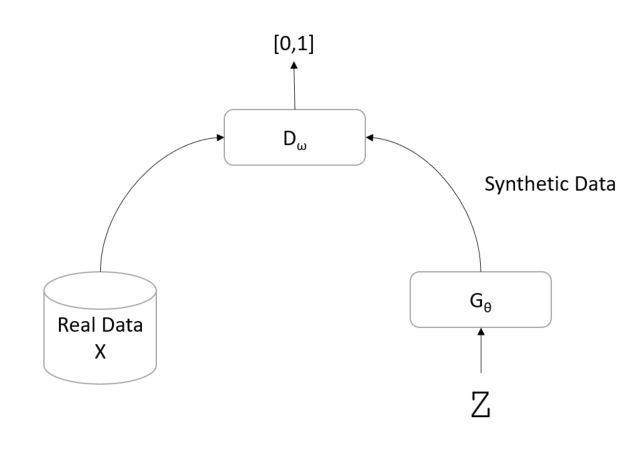
\includegraphics[width=\textwidth]{image.png}
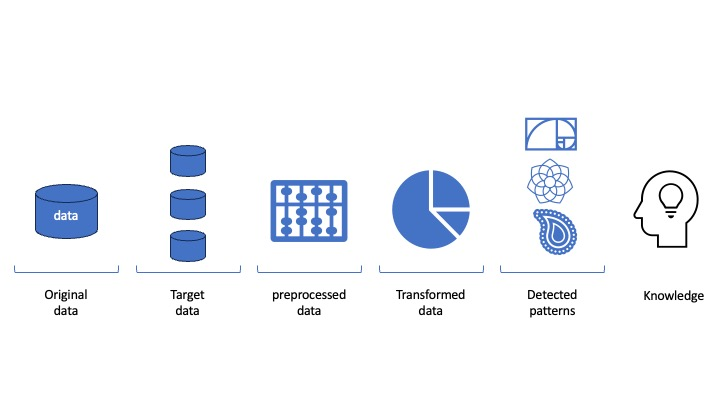
\includegraphics[scale=0.55]{figures/imagens-tese.jpg}

\caption{\acl{kdd} Process, adapted from \cite{Fayyad_Piatetsky-Shapiro_Smyth_1996}} \label{fig:kdd-generic}
\end{figure}

Several frameworks have been proposed to implement the \ac{kdd} process. One such prominent framework is \ac{crispdm}, which comprises business understanding, data understanding, data preparation, modelling, evaluation, and deployment. \ac{crispdm} was conceived in 1996 and became a \ac{eu} project under the ESPRIT funding initiative in 1997 \cite{Chapman2000CRISPDM1S}. \ac{semma} \cite{rohanizadehProposedDataMining2009} involves five stages: sampling, exploration, modification, modelling, and assessment. It starts by analysing a subset of data, then seeks patterns and modifies variables. A model is built, and the results are evaluated. While SEMMA covers key data-mining aspects, it misses fundamental components of information system projects like analysis and implementation.

It is important to distinguish however that \ac{kdd} is not the same as Data Mining. Like stated in \cite{Fayyad_Piatetsky-Shapiro_Smyth_1996}, we agree that \ac{kdd} is a major process of which Data Mining is a part. So, in order to understand the process of \ac{kdd}, we need to understand the process of Data Mining, which can be understood as the application of algorithms for extracting patterns from data. There are several classes of algorithms, each best suited for different kinds of tasks:
\begin{itemize}
    \item Classification Algorithms: These are used to predict categorical class labels. Examples include Decision Trees, Naive Bayes, \ac{svm}, \ac{knn}, and various types of Neural Networks. These are used in disease diagnosis, patient risk prediction, and readmission prediction.
\item Clustering Algorithms: These are unsupervised methods used to group similar data points together. K-Means, Hierarchical Clustering, DBSCAN, and Self-Organizing Maps are common clustering algorithms used in patient segmentation and anomaly detection.

\item Regression Algorithms: These are used to predict continuous output variables. Examples include Linear Regression, Logistic Regression, and Regression Trees. These algorithms find application in predicting disease progression and healthcare costs.

\item Association Rule Mining Algorithms: These discover associations or patterns among a set of items in large databases. \textit{Apriori} and FP-Growth are commonly used algorithms in this class, helping in discovering co-occurring health conditions or drug interactions.
\item Sequential Pattern Mining Algorithms: These help discover or predict specific sequences of events, which is particularly useful in medical trajectory analysis.

\item More sophisticated architectures and algorithms appeared with neural networks, generative \ac{ai}, and reinforcement learning, among others.

\end{itemize}

As a result, \ac{kdd} is the process of applying Data Mining algorithms to data but also the data preparation, selection, cleaning, and most important of all, the incorporation of prior knowledge about the domain along with the proper interpretation of results. This difference is vital to understanding \ac{kdd} since blindly applying data mining or \ac{ml} methods to data will only render results that are not useful or even misleading \cite{Fayyad_Piatetsky-Shapiro_Smyth_1996}.

In short, \ac{kdd} can be understood as a multidisciplinary subject that bridges and aggregates knowledge from different areas like \ac{ml}, pattern recognition, databases, statistics, AI, knowledge acquisition for expert systems, data visualization, and high-performance computing. On top of all of these subject and research areas, sits the most important of all - which is domain expertise.
%-tipos de algortimos paraa

